% assignment_3.tex
% CS 8725 - Supervised Learning (Fall 2015)
%     University of Missouri-Columbia
%             Chanmann Lim
%            September 2015

\documentclass[a4paper]{article}

\usepackage[margin=1 in]{geometry}
\usepackage{listings}
\usepackage{amsmath}
\usepackage{amsfonts}
\usepackage{graphicx}
\usepackage{float}
\usepackage{multirow}

\everymath{\displaystyle}
\DeclareMathOperator*{\argmax}{\arg\!\max}
\DeclareMathOperator*{\argmin}{\arg\!\min}

\begin{document}
\title{CS 8725: Report for assignment 3}
\author{Chanmann Lim}
\date{September 28, 2015}
\maketitle

\noindent
	The Matlab code for all experiments is in the \textbf{Appendix} section.

\paragraph{Programming 1:} We are given a bunch of data samples of "Average height and weight of American women aged 30 to 39" and the task is to design linear regression algorithm to predict the $ weight \in \mathbb{R}$ denoted by $Y$ from a given height measurement denoted by $X$ then the problem becomes $f(X) \to Y$ finding a function mapping from X to Y. In linear regression we assume that $f(X)$ take a linear form with respect to $X$ that is $f(X) = \beta_1 + \beta_2X$ and the goal is to choose $\hat{f}(X)$ that minimizes the prediction error (squared error). \\

	\begin{equation}
		\hat{f}_n^L = \argmin_f \frac{1}{n} \sum_{i=1}^n (f(X_i) - Y_i)^2
	\end{equation}

	By rewriting $f(X)$ in term of $\beta = [\beta_1\; \beta_2]^T$, minimizing $f(X)$ becoming minimizing $\beta$.
	
	\begin{align}
		\hat{\beta} &= \argmin_{\beta} \frac{1}{n} \sum_{i=1}^n (X_i\beta - Y_i)^2\\
			&= \argmin_{\beta} \frac{1}{n} (A\beta - Y)^T(A\beta - Y)  \label{eq:beta_hat}
	\end{align}
	
	Where, 
	
	\begin{equation}
		A = \begin{bmatrix} 
				1 & X_1 \\ 
				\vdots & \vdots \\ 
				1 & X_n 
			\end{bmatrix} \text{ and }
		Y = \begin{bmatrix} 
				Y_1 \\ 
				\vdots \\ 
				Y_n 
			\end{bmatrix}
	\end{equation}
	
	If we define $J(\beta) = (A\beta - Y)^T(A\beta - Y)$ then minimizing $J(\beta)$ is equivalent to \eqref{eq:beta_hat}.
	
	\begin{align}
		\frac{\partial J(\beta)}{\partial \beta} &= \frac{\partial A^TA\beta\beta^T - 2\beta^TA^TY - Y^TY}{\partial \beta} \\ 
			&= 2A^TA\beta - 2A^TY
	\end{align}
	
	\begin{align}
		2A^TA\hat{\beta} - 2A^TY &= 0 \\ 
		A^TA\hat{\beta} &= A^TY \\ 
		\hat{\beta} &= (A^TA)^{-1}A^TY \label{eq:normal_eq}
	\end{align}
	
	Eq. ~\eqref{eq:normal_eq} is the normal equation with $(A^TA)$ as normal matrix and $\hat{f}_n^L = X\hat{\beta}$. As a result we obtained the linear regression coefficient in \eqref{eq:beta_hat_value} and the expected error in \eqref{eq:risk_1}:
	
	\begin{equation} \label{eq:beta_hat_value}
		\hat{\beta} = [-39.0620 \quad 61.2722]^T
	\end{equation}
	
	\begin{align}
		R(\hat{f}) &= \mathbb{E}[(\hat{f}(X) - Y)^2] \\ 
			&= \frac{1}{n} (X\hat{\beta} - Y)^T(X\hat{\beta} - Y) \\
			&= 0.4994 \label{eq:risk_1}
	\end{align}
	
	In fact for this case in particular, we know that we could further reduce the expected error $R(\hat{f})$ by introducing quadratic term into the regression. With this procedure we have turned linear regression into polynomial regression and by following the derivation in solving for $\hat{\beta}$ it turn out that $\hat{\beta} = (A^TA)^{-1}A^TY$ where $\beta = [\beta_1\;\beta_1\;\beta_3]^T$ and 
	$$ A = \begin{bmatrix} 
				1 & X_1 & X_1^2 \\ 
				\vdots & \vdots & \vdots \\ 
				1 & X_n & X_n^2
			\end{bmatrix}$$
			
	We obtained $\hat{\beta} = [128.8128 \quad -143.1620 \quad 61.9603]^T$ and $R(\hat{f}) = 0.0506$ for second order polynomial regression. Figure ~\ref{fig:regression} show the both linear and polynomial regression functions with respect to the data samples.
	
	\begin{figure}[H]
		\centering
		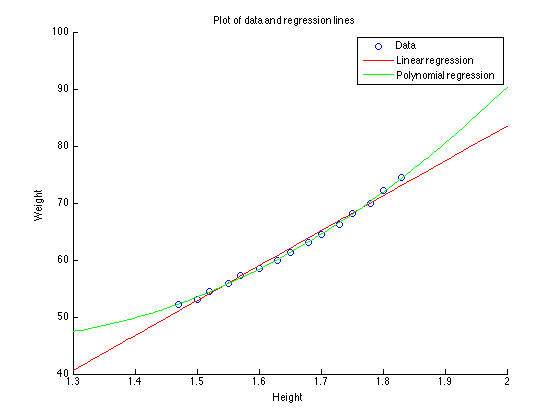
\includegraphics[scale=.57]{images/regression.png}
		\caption{Plot of data and regression lines}
		\label{fig:regression}
	\end{figure}
\newpage
\subsection*{Appendix:}
	\lstinputlisting[language=Matlab, title=\lstname, basicstyle=\footnotesize]{assignment_3.m}
	\lstinputlisting[language=Matlab, title=\lstname, basicstyle=\footnotesize]{problem_1.m}
	\lstinputlisting[language=Matlab, title=\lstname, basicstyle=\footnotesize]{problem_2.m}
\end{document}